\documentclass{article} 
\usepackage{tikz}
\usetikzlibrary{chains}
\usepackage[utf8]{inputenc}
\usepackage[T1]{fontenc}
\usepackage{lmodern}

\begin{document}

\begin{enumerate}
\item

\begin{tikzpicture}[start chain, 
    every node/.style={on chain},
    bloc/.style={fill=red!80!blue!70, 
        minimum width=3.5cm, minimum height=1.2cm, 
        text=white, font=\sffamily, align=center,   
        outer sep=0pt},
    simbol/.style={text=blue!80, 
        font=\bfseries\Large, outer sep=0pt},
    node distance=0pt,
    ]
    \node[bloc] {Gasto en\\ pensiones};
    \node[simbol] {=};
    \node[bloc, fill=green!80!black] {Ingresos del sistema de \\ pensiones};
\end{tikzpicture}

\item

\begin{tikzpicture}[start chain, 
    every node/.style={on chain},
    bloc/.style={fill=red!80!blue!70, 
        minimum width=1.8cm, minimum height=1.5cm, 
        text=white, font=\sffamily, align=center,   
        outer sep=0pt},
    simbol/.style={text=blue!80, 
        font=\bfseries\Large, outer sep=0pt},
    node distance = 0pt
    ]
    \node[bloc] {IRP};
    \node[simbol] {+};
    \node[bloc] {Crecimiento\\ número de \\ pensiones};
    \node[simbol] {+};
    \node[bloc] {Efecto\\ sustitución\\ (altas/bajas)};
    \node[simbol] {=};
    \node[bloc, fill=green!80!black] {Inflación};
    \node[simbol] {+};
    \node[bloc, fill=green!80!black] {Crecimiento\\ real de los\\ ingresos};
\end{tikzpicture}

\item

\begin{tikzpicture}[start chain,
    every node/.style={on chain},
    bloc/.style={fill=red!80!blue!70, 
        minimum width=1.7cm, minimum height=1.5cm, 
        text=white, font=\sffamily, align=center,   
        outer sep=0pt},
    simbol/.style={text=blue!80, 
        font=\bfseries\Large, outer sep=0pt,
        minimum height=1.5cm},
    node distance = 0pt
    ]
    \node[bloc] {IRP};
    \node[simbol] {=};
    \node[bloc, fill=blue!30] {Inflación};
    \node[simbol] {+};
    \node[bloc, fill=blue!30] {Crecimiento\\ real de los\\ ingresos};
    \node[simbol, fill=blue!30] {-};
    \node[bloc, fill=blue!30] {Crecimiento\\ número de \\ pensiones};
    \node[simbol, fill=blue!30] {-};
    \node[bloc, fill=blue!30] {Efecto\\ sustitución\\ (altas/bajas)};
\end{tikzpicture}

\item
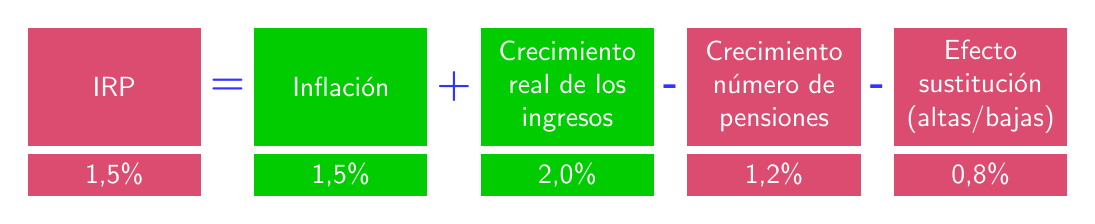
\begin{tikzpicture}[start chain,
    bloc/.style={fill=red!80!blue!70, 
        minimum width=2.2cm, minimum height=1.5cm, 
        text=white, font=\sffamily, align=center,   
        outer sep=0pt},
    simbol/.style={text=blue!80, 
        font=\bfseries\Large, outer sep=0pt},
    lbl/.style={text=white, font=\sffamily, 
        align=center, outer sep=1mm,
        minimum width=2.2cm, fill=red!80!blue!70},
    node distance = 0pt
    ]
    \node[on chain, bloc, 
        label={[lbl]below:1,5\%}] {IRP};
    \node[on chain, simbol] {=};
    \node[on chain, bloc, fill=green!80!black, 
        label={[lbl,fill=green!80!black]below:1,5\%}] {Inflación};
    \node[on chain, simbol] {+};
    \node[on chain, bloc, fill=green!80!black,
        label={[lbl,fill=green!80!black]below:2,0\%}] {Crecimiento\\ real de los\\ ingresos};
    \node[on chain, simbol] {-};
    \node[on chain, bloc,
        label={[lbl]below:1,2\%}] {Crecimiento\\ número de \\ pensiones};
    \node[on chain, simbol] {-};
    \node[on chain, bloc,
        label={[lbl]below:0,8\%}] {Efecto\\ sustitución\\ (altas/bajas)};
\end{tikzpicture}
\end{enumerate}
\end{document}